% This work is licensed under the Creative Commons Attribution 4.0 International License. To view a copy of this license, visit http://creativecommons.org/licenses/by/4.0/ or send a letter to Creative Commons, PO Box 1866, Mountain View, CA 94042, USA.

\documentclass[12pt, twoside]{report}
% Use package to keep preamble setup
\usepackage{architecture}

\begin{document}
\title{Complexes Manual}

\thispagestyle{plain}
\begin{center}
    \Large
    \textbf{Complexes Code Architecture}
       
    \vspace{0.9cm}
    \textbf{Abstract}
\end{center}

This document is intented for people who want to extend complexes or understand the 
code in more detail. The code is described at a high level outlining the general
ideas and design.

\tableofcontents

\chapter{\complexes}

\complexes is a Monte Carlo simulation engine implementing the complexes protein
model. The program is written in modern \mbox{C++14} with a focus on being
extensible. The program contains an extensible Monte-Carlo engine, the modified
Lennard-Jones potential, \cref{eq:ch5:complexesLJ} and other pair potentials,
the Monte-Carlo movements for different domain types, and a cell-list algorithm
\cite{frenkel2001understanding} to speed up the energy evaluations.


\section{Flexible and Extensible Core Algorithms}

The core algorithms of the Monte-Carlo engine have the ability to add new trial
moves for domains and to add new Monte-Carlo algorithms for different
statistical ensembles or enhanced sampling techniques. This extensibility is
achieved thought a combination of run-time polymorphism and use of modern
\mbox{C++14}. In \complexes, this technique is used to implement domain trial
moves, Monte-Carlo algorithms, evaluation of pair potentials, and a cell-list
algorithm. In \mbox{C++} run-time polymorphism is implemented through abstract
classes and inheritance. In \complexes abstract classes are marked with the
preposition ``Abstract''. The most interesting abstract classes to add new
features to \complexes are \inlinecode{AbstractDomain},
\inlinecode{AbstractPairKernel}, \inlinecode{AbstractConnection},
\inlinecode{AbstractInteractionGrid} and \inlinecode{AbstractMcAlgo}. See
\cref{fig:Complexes} for a schematic how these classes interact with each other
during a simulation.
\begin{figure}[!ht] \centering
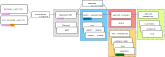
\includegraphics[width=\textwidth]{figures/software-model}
\caption[Complexes software overview.]{Schematic of the classes used in the
\complexes program and how they interact with each other (arrows). Abstract
classes and their explicit implementations are shown as colored boxes. Nested
boxes show different implementations of an abstract class. Names are as in the
code.}
\label{fig:Complexes}
\end{figure}

\section{Monte-Carlo Algorithm}

The main logic to run a Monte-Carlo simulation is implement in
\inlinecode{AbstractMcAlgo} with a virtual method called \inlinecode{sweep} to
implement a sweep. Currently \complexes implements sweep functions for the NVT
and N\(\Pi\)T ensemble \cite{frenkel2001understanding}. In addition two
different acceptance functions, Metropolis \cite{metropolis1953} and Glauber
\cite{Glauber1963} have been implemented as well. All Monte-Carlo sweep
algorithms work with all acceptance functions.

For a sweep in the NVT ensemble domains are chosen randomly from a uniform
distribution. If \(N\) is the number of domains that than a sweep will make
\(N\) trial moves and select a random domain with probability \(1/N\) for each
trial. In the N\(\Pi\)T ensemble trial moves are generated for the domains and
the volume. To account for the additional volume move a sweep consists of
\(N+1\) trial moves. At each trial, the probability to make a volume move is
\(1/(N+1)\). If a domain move was chosen the domain to be moved is chosen
randomly with a \(1/N\) probability. For the volume moves the domains are
re-scaled so that the centroid of the domain is scaled by
\(\sqrt[3]{(V+dV)/V}\). The N\(\Pi\)T algorithm is called NPT in the code and
configuration files.

\section{Boundary Conditions}

\complexes treats boundary effects using periodic boundary conditions
\cite{frenkel2001understanding}. Under these conditions, the centroid of all
domains is placed inside of the unit-cell. \complexes only implements
rectangular unit-cells. Because \complexes keeps the centroid of a domain within
the box it can happen that some beads are outside of the box.

To determine the distance between two beads \complexes uses the \gls{MIC}
\cite{frenkel2001understanding}. \complexes uses an efficient implementation to
calculate the minimum image distance, \cref{algo:fast-mic}. This algorithm is an
extension of a fast algorithm \cite{Deiters2013}, where the while-loop ensures
it works for any distance to ensure the algorithm will also work if trial moves
displace a domain by more than one periodic image. To ensure that the number of
iterations of the while-loop are as small as possible \complexes ensures that
the centroid of a domain are inside the unit-cell.
\begin{algorithm2e}[h!] \SetAlgoLined \DontPrintSemicolon \Fn{mic(distance[3],
box[3])} { \For{i=0; i<3; ++i}{ \While{distance[i] > .5 * box[i]} { distance[i]
-= box[i]\; } \While{distance[i] < .5 * box[i]} { distance[i] += box[i]\; } }
return distance; }
  \caption{Algorithm to efficiently convert the distance between two beads to
the minimum image distance it domain centers are inside of the simulation box.}
 \label{algo:fast-mic}
\end{algorithm2e}

\section{Replica Exchange Algorithms}

The theoretical descriptions of the replica exchange algorithms do not specify
which replicas are exchanged in an attempt. To increase the probability to
accepted an exchange attempt in complexes only neighboring replicas are
exchanged \cite{Bussi2014}. During an exchange, not all neighboring pairs are
attempted to exchange, this is because the exchange between replica \(i\) and
\(i+1\) also depends on replica \(i-1\). Rather in \complexes attempts are only
done between even pairs when the attempt number is even and odd pairs otherwise.
In an even pair, of replicas \(i\) and \(i+1\), then \(i\) is even and odd for
odd pairs. For consistency 0 is counted as an even number and 1 as an odd
number.

Replica simulations require that multiple simulations are started. \complexes
requires that every replica is started in its own folder. Multiple simulations
can be started with the \inlinecode{--multidir} flag and a list of the folders
containing individual replicas. The \inlinecode{--multidir} option alone only
tells complexes to simulate multiple replicas to activate the exchange two flags
\inlinecode{--replex} and \inlinecode{--replex-accept} have to be used as well.
\inlinecode{--replex} states after how many sweeps an exchange should be
attempted. \inlinecode{--replex-accept} states the exchange function to be used.

The replica exchange simulations are also implemented in an extensible manner.
Because the different replicas exchange algorithms implemented require different
variables to be changed between the replicas, \complexes only exchanges the
coordinates of the beads and box dimensions during an exchange.


\section{Random Numbers}
\complexes uses pseudo random numbers to generate trial moves and accept moves.
As a pseudo \gls{RNG} it is using the mersenne twister \cite{Matsumoto1998}
implementation in the C++ standard library. Because the \gls{RNG} cannot be
safely used in a multi-threaded program like \complexes it uses a different
instance of the \gls{RNG} for each thread. The individual \gls{RNG} instances
are seeded from random numbers from an initial \gls{RNG} instance during setup.
To achieve reproducability \complexes requires the user to provide an explicit
seed for the initial \gls{RNG}. This requirement ensures that two runs with the
same input are identical on the same computation node.

\section{Pair Interactions Potentials}

The different pair kernels are implemented with a common abstract base class
\inlinecode{AbstractPairKernel}. The Lennard-Jones like and \gls{WCA} potential
have been implemented using Inastemp, a portable \gls{SIMD} library,
\cite{Bramas2017}.

\section{Bead and Domain Implementation}

No specific bead class exists in \complexes, instead, domains contain all
information specific to the beads as several lists. This design scheme follows
the ``struct of arrays'' pattern \cite{wikiAOS} used to optimize memory access.
For the beads a domain stores the coordinates in a \inlinecode{m\_xyz} field,
the charges in \inlinecode{m\_charges} and the bead types in
\inlinecode{m\_beads}. These three fields are the only information needed to
evaluate the potential energy with the pair potential functions. Domains are
also implemented with run-time polymorphism in an AbstractDomain class that
contains information about the beads and coordinates. Derived classes only need
to implement trial moves.

In addition to bead information, a domain also contains a unique id and a type
id that are defined at runtime. The type id is used to find the corresponding
pair kernel when evaluating the energy with a different domain. Choosing a
pair-kernel for domain type pairs and using a struct of arrays pattern allows
evaluating the pair-kernel for groups of beads. This pattern can be efficiently
implemented using inastemp \cite{Bramas2017}. Because the evaluation of the
pair-kernel is the most expensive calculation of \complexes this pattern ensures
that \complexes has good performance while using run-time polymorphism. The type
ids are also used to create domains with the same type of move but different
parametrizations for it. For example, the rigid domains have two parameters for
translation and rotation. Having the final parametrization set at runtime allows
creating two distinct rigid domain types for different proteins. This
flexibility is useful for simulations with a mixture of small and large domains.
The translation and rotation of larger domains can be chosen smaller to increase
the acceptance rate for their moves and small domains can be set to large
translation and rotation. Allowing to achieve optimal phase space exploration
rate for a simulation.

In \complexes only the rigid domain types is implemented. For the Monte-Carlo
moves the rigid domains can be translated by an arbitrary vector, each component
is chosen randomly from the range \([-a, +a]\), with \(a\) the maximal
displacement. The rotations are generated by choosing a random rotation axes in
the unit cube and a random rotation angle \cite{frenkel2001understanding}. This
method generates a known artifact that rotation axes along the edges are over
sampled. Because the all edges are equally sampled it does not affect generated
ensembles. In each trial move the probability to make a translation or a
rotation move is one half.

\section{Flexible Linkers and Connection Potentials}
As described in the theory flexible linker domains are replaced with effective
potentials from a Gaussian chain polymer model. For this \complexes implements
connection potentials in a \inlinecode{Connection} class. A connection contains
the ids of the two domains that are connected and the corresponding bead ids in
the domains. For each domain, a list of connections is stored in the class. So
if domains \(i\) and \(j\) are connected both contain the same connection. This
duplication of data makes it easier finding the corresponding connections for a
domain during the energy calculation. This compromise was chosen as it is
expected that the number of connections is significantly smaller the number of
beads. Currently implemented connection potentials are a flat potential (zero
everywhere), a harmonic potential, and a Gaussian chain \gls{PMF} potential,
\cref{eq:ch5:PMF-complexes}.

\section{Cell List Algorithm}

The other important part of the performance of complexes is the cell list
algorithm \cite{frenkel2001understanding} used to reduce the number of
interactions needed to evaluate. Cell-list algorithms reduce the computation
time to calculate the full energy from \(\mathcal{O}(N^2)\) to
\(\mathcal{O}(N)\) with \(N\) being the number of beads in a simulation. The
algorithm stores for every cell continues intervals of beads that are in the
corresponding cell. Every bead in a domain is given a unique id defined by the
order in which they appear in the input files. The interval will therefore only
store the id of the first bead entering the cell and the length of beads in the
cell. For domains that are larger than a single cell it can happen that two
different intervals are in a cell, see the red domain in
\cref{fig:celllist-datastructure} that has two intervals in the cell (1, 4). In
that case, the cell will store two intervals for the same domain. An intervals
is stored in the \inlinecode{CoInterval} class, \cref{listing:c++-celllist}.
Each cell stores a list of CoInterval instances. As an example of the data
stored for a list take the cell (1, 4) containing the red domain in
\cref{fig:celllist-datastructure}.
\begin{listing}[!ht]
  \begin{minted}{c++}
    class CoCell {
      // The list of intervals inside the current
      cell std::vector<CoInterval> m_intervals;
      // ...
    };

    class CoInterval {
      // The domain related to the current interval
      int m_domainId;
      // The position of the first element of the element-list
      int m_beginingOfInterval;
      // The number of elements in the current interval
      int m_nbElementsInInterval;
      // ...
    };
\end{minted}
\caption{Definition of the CoCell and CoInterval class used in the cell list
algorithm implemented in \complexes. The comment ``\inlinecode{...}'' indicates
other implementation details.}
\label{listing:c++-celllist}
\end{listing}
\begin{figure}[!ht] \centering
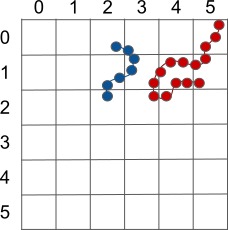
\includegraphics[]{figures/Complexesppintervals}
\caption[Cell list data-structure example.]{Example configuration for two
domains (blue and red) in a 2D grid. Numbers on the top and left are used to
index cells.}
\label{fig:celllist-datastructure}
\end{figure}

To calculate the completely potential energy between all domains we iterate over
all cells in the cell-list, see \cref{algo:cell-list}. For each cell we then
iterate over the list of CoIntervals.
\begin{algorithm2e}[h!] \SetAlgoLined \DontPrintSemicolon
  \Fn{computeEnergy(Cells[K], Domains[M])} { energy = 0\; \tcp{Compute energy
      (particle to particle interactions)} \For{cell \textbf{in} Cells}{
      \For{target \textbf{in} cell}{ \For{source \textbf{in} cell}{
          \If{source.domainId $\neq$ target.domainId}{ target\_dom =
            Domains[target.domainId]\; source\_dom = Domains[source.domainId]\;
            energy += kernel(target\_dom, source\_dom, target, source)\; } }
        \For{nb\_cell \textbf{in} cell.neighbors()}{ \For{source \textbf{in}
            nb\_cell}{ \If{source.domainId $\neq$ target.domainId}{ target\_dom
              = Domains[target.domainId]\; source\_dom =
              Domains[source.domainId]\; energy += kernel(target\_dom,
              source\_dom, target, source)\; } } } } } return energy }
 \caption{Cell list algorithm to calculate all pair interactions.}
 \label{algo:cell-list}
\end{algorithm2e}
During a Monte Carlo move only a single domain will be moved.
We therefore do not need to recalculate the complete potential energy. Instead
we need iterate over the cells occupied by the moved domain and update the
energy difference appropriately, replacing the outer most loop in
\cref{algo:cell-list} with a loop over only the cell currently occupied by the
domain. The last step further reduces the computational effort to calculate
energies during a simulation.

The interface to the cell list algorithm to calculate pair interactions has also
been implemented without references to the underlying algorithm and can be
swapped out with different algorithms. In \complexes, there are two
data-structures available for the cutoff grid. The \textit{dense} data structure
is allocated cell objects for all cells in a simulation box and offers efficient
computation of neighboring cells. The memory consumption of this data structure
scales with \((L_{\mathrm{Box}}/L_{\mathrm{Cell}})^3\), where
\(L_{\mathrm{Box}}\) is the edge-length of the simulation box and
\(L_{\mathrm{Cell}}\) is the edge-length of a cell, see
\cref{fig:container-memory-scaling}. This data structure is optimal for dense
simulations. The \textit{sparse} data structure uses a hash-map to only allocate
cells that are occupied by beads. The memory consumption of this data structure
scales with the number of beads in a simulation and is independent of the box
size. It is suited for sparse simulations. The high-level interface is also
agnostic to the underlying cell-list algorithm allowing to chose a completely
different algorithm if desired.
\begin{figure}[!ht]
  \centering
  \includegraphics{figures/container-memory-scaling}
  \caption{Memory consumption of the dense (blue) and sparse (orange) cell-list
    data-structure with a constant number of beads. The cutoff is set to
    \SI{12}{\AA}. The gray line marks one gigabyte.}
\label{fig:container-memory-scaling}
\end{figure}

\section{Task based parallelism}

Monte Carlo algorithms have two points which can be parallelized, the energy
calculation and the trial move generation. The trial move generation in
complexes is not computationally expensive and a minuscule amount of time is
spend on it. Leaving the energy calculation for the single replica simulations.
In replica exchange Monte-Carlo all replicas can be executed in parallel with
few synchronization points to exchange coordinates. Ideally, the single replica
and replica exchange simulation can use the same parallelisms scheme. It has to
be taken into account that replicas can be unbalanced or change during a
simulation if a phase transition occurs (from liquid to solid). Another
requirement was that it should be possible to always use the maximal number of
available \gls{CPU} cores independent of the number of replicas. Meaning a
single replica can use multiple threads and in the case that more replicas than
available threads are simulated the different replicas have a scheduler queue.

In \complexes this problem is solved using the task \gls{API} in OpenMP
\cite{openMP}. Tasks are generated based on either domains or cell lists (if
activate). Meaning tasks are small and plentiful. At the beginning of the energy
calculation, the number of tasks is distributed equally to the available
threads. If a thread finishes early it can then steal tasks from other threads.
Allowing threads to be always busy. It balances when different replicas have
different work loads. Nothing special is done to minimize the numa effect.
Therefore, it is maybe better to one process per memory node (explicit sync) and
threads inside.

The replica simulations can run in parallel. To make better use of available
resources that allow multi-node jobs also a \gls{MPI} implementation has been
developed. There is no work stealing between replicas in this configuration.

\section{\cplx File Format}

The input for \complexes simulation is stored in a \cplx file similar to the tpr
files in GROMACS. The \cplx file contains all information about the domains and
pair kernels to simulate, with the exception of the parameters for the
Monte-Carlo algorithm and the used forcefield parameters. The \cplx file format
is based on \yaml\cite{YAML} and divided into four sections \textit{box,
definitions}, \textit{topologies}, and \textit{forcefield}.

The \textit{box} section contains the dimensions of the rectangular simulation
box as a \yaml list. The length in each dimension is given in \SI{}{\AA}.

The \textit{definitions} section defines the type of domains that are used in
the simulation and the pair kernels used to calculate the energy between
domains. The \textit{definitions} section is separated into two sub sections to
define the final domain-types and their interactions between them, called
\textit{domains} and \textit{pair-interactions} respectively. The
\textit{domains} section contains a dictionary with the entry names being the
domain names and the definition for the domain. A definition contains the type
of move the domain can make, currently only rigid is implemented, and the parameters for
the move. Allowing to define several rigid bodies in a simulation that have
different rotation and translation parameters. The definitions can be used for
systems with a mixture of large and small rigid bodies to model the
corresponding mobility. The \textit{pair-interaction} section defines which pair
interaction potential to choose for each combination of domain types defined in
\textit{domains}. In the definition, one can define more domain types than what
will be used in a simulation. Allowing to create standard definitions (like the
\gls{KH} forcefield) for different applications. See
\cref{listing:cplx-definitions} for an example definition using two domain types
\textbf{A} and \textbf{EM}. Here the \textbf{EM} type is set to not move at all
and interacts with \textbf{A} domains using the \gls{WCA} potential. This
definition could be used to fit any domain of type \textbf{A} into a domain
defined by \textbf{EM}.
\begin{listing}[!ht]
  \begin{minted}{yaml}
    definitions:
      domains:
        A:
          defaults: {rotation: 2, translation: 1}
          move: rigid
       EM:
          defaults: {rotation: 0, translation: 0}
       move: rigid
    pair-interaction:
      - domain-type-pair: [A, EM] function: WCA
      - domain-type-pair: [A, A] function: LJH
      - domain-type-pair: [EM, EM] function: None
\end{minted}
\caption{\complexes domain definitions for a simulation with two domain types
\textbf{A} and \textbf{EM}. Both domain types move as rigid bodies but they have
different pair interaction potentials with each other.}
\label{listing:cplx-definitions}
\end{listing}

The \textit{topologies} section defines the actual domains that are used in the
simulation. It consists of a \yaml list of topology entries. Each topology entry
contains domain definitions and connections between domains of the same
topology. A domain contains the following field: beads, chain-ids, charges,
coordinates, nbeads, type, mc-moves, meta-data, name. Here the type field
specifies the domain type, which has to be defined in the definitions section.
Domains have to be numbered consecutively and uniquely across all topologies.

The \textit{forcefield} section contains definitions for the available bead
types as well as the energy and diameter pair parameters.

\chapter{\pycomplexes}
\begin{listing}[!ht]
  \begin{minted}{yaml}
    box: [100, 100, 100]
    topology:
      protein-name:
        coordinate-file: structure.pdb
        move: true
        domains:
          A:
            type: rigid
            selection: 'namd CA and segid A'
          link:
            type: gaussian
            selection: 'name CA and segid L'
            start_connection: [A, 'segid A and resid 10']
            end_connection: [B, 'segid B and resid 10']
          B:
            type: rigid
            selection: 'name CA and segid B'
\end{minted}
\caption{TOP file for a simulation for two rigid domains connected by a Gaussian
domain. All selections are written in the atom selection language used by
MDAnalysis.}
\label{listing:top-definitions}
\end{listing} pycomplexes is a \mbox{Python} library and \gls{CLI} program that
includes several tools to help setup simulations for \complexes and analyze them
later. The \cplx format accepted by \complexes is very complex and allows the
user a lot of freedom in setting up the simulation. A lot of simulation setups
do not need to leverage the full flexibility of complexes and therefore
pycomplexes includes a tool called \inlinecode{convert} that takes as input a
simplified format, called a TOP file, for describing simulations and generating
\cplx files from it. As part of the conversion, the script will automatically
choose charges and interaction energies based on amino acid type. As interaction
energies, the user can choose either the \gls{KH} model or the unaltered
\gls{MJ} model. The charges are set according to the \gls{KH} model in both
cases. The interaction potential is chosen based on domain type, so far allowed
are rigid and gaussian. The rigid domain type uses the modified lennard jones
potential, \cref{eq:ch5:complexesLJ}. For the gaussian domains positions of the
\calpha beads will be stored in the \cplx as rigid domains that do not move and
a connection potential, \cref{eq:ch5:PMF}, will be used between the two rigid
domains connected by the gaussian domain. To define a domain in the top file the
type and a selection of beads have to be specified. For the gaussian domain, in
addition, the beads of the rigid domains connected by the gaussian domain have
to be specified as well. The convert script could ignore known beads for a
gaussian domain in the structure but keeping the information in the \cplx file
allows to generate explicit linker positions in the post processing, i.e. with
the \inlinecode{addlinker} tool.

The structures and selections are read and parsed using
MDAnalysis\cite{oliver_beckstein-proc-scipy-2016, Michaud-agrawal2011}. In the
molecular dynamics community there exists a large variety of structure file
format and they are often not well defined or popular programs write and accept
ill formatted files, MDAnalysis helps to read a large variety of different
formats with an easy to understand atom selection language.

In addition to the \inlinecode{convert} command pycomplexes also include a
variety of other commands to help the user setup and visualize simulations. As
of the time of writing the other implemented commands are
\begin{itemize}
  \item \inlinecode{equilibration} Update coordinates stored in a CPLX from a
trajectory.
  \item \inlinecode{forcefield} Convert a forcefield using scaling parameters
\(\lambda\) and \(e_0\), see \cref{eq:ch5:complexesEpsilon}.
  \item \inlinecode{visualize} Create VMD scripts from simulations.
  \item \inlinecode{demux} generate input files for the GROMACS tool
\inlinecode{trjcat} to generate time-continuous trajectories from replica
exchange simulations.
  \item \inlinecode{addlinker} generate explicit linker conformations for a
simulation with Gaussian linkers.
\end{itemize}



\clearpage
%%%%%%%%%%%%%%%%
% BIBLIOGRAPHY %
%%%%%%%%%%%%%%%%
\phantomsection
\addcontentsline{toc}{chapter}{Bibliography}
\bibliography{manual}
\clearpage
\printglossary[type=\acronymtype,title=List of Abbreviations]
\end{document}
